%& -shell-escape
\documentclass[a4paper,11pt]{book}
\usepackage[ruled,boxed]{algorithm2e} 
\usepackage[fleqn,reqno]{amsmath}
\usepackage{amsfonts}
\usepackage{amssymb}
\usepackage{a4wide}
\usepackage{graphicx}
\usepackage{fancyhdr}
\usepackage[utf8]{inputenc}
\usepackage[french,english]{babel}
\usepackage{natbib} %% citations
\usepackage{hyperref}
\usepackage{caption}
\usepackage{subfigure}
\usepackage{color} 
\usepackage{xspace}
%%\usepackage{slashbox} %% no longer in texlive
\usepackage{diagbox} %% replacement
\usepackage{pdfpages}
\usepackage{marvosym}
\usepackage{anysize}
\usepackage{makeidx}
\usepackage{xspace}
\usepackage{fancyvrb, listings, color}
\usepackage[usenames,dvipsnames,svgnames,table]{xcolor}
%%
\usepackage{python}

%%% Python (kind of important)
\lstloadlanguages{Python}

\definecolor{gogetit}{HTML}{6C8B9F}


%%% Margins

\marginsize{2cm}{2cm}{2cm}{2cm}

%%% indexation
\makeindex

%%% very strange missing counter within pdflatex
\newcounter{Hy@AnnotLevel}

%% a real new counter for custom python listings
\newcounter{codein}
\setcounter{codein}{0}
\newcommand{\pylabel}[1]{\refstepcounter{codein}\label{#1}}

%% fraction texte sur figure moins conservatrice
\renewcommand{\topfraction}{.85}
\renewcommand{\bottomfraction}{.7}
\renewcommand{\textfraction}{.15}
\renewcommand{\floatpagefraction}{.66}
\renewcommand{\dbltopfraction}{.66}
\renewcommand{\dblfloatpagefraction}{.66}

%%%%%%%%%%%%%% Useful macros %%%%%%%%%%%%%%%%%%%%%%%%%%

\newenvironment{myitem}{\begin{list}{$\bullet$}{\partopsep 0pt plus 1pt
\topsep 0pt plus 1pt \itemsep 0pt \labelwidth 5pt}}{\end{list}}

\newenvironment{myit}{\begin{list}{$-$}{\partopsep 0pt plus 1pt
\topsep 0pt plus 1pt \itemsep 0pt \labelwidth 5pt}}{\end{list}}

\catcode`\@=11\relax
\def\rightarrowfill{$\m@th \mathord- \mkern-6mu
  \cleaders\hbox{$\mkern-2mu \mathord- \mkern-2mu$}\hfill
  \mkern-6mu \mathord\rightarrow$}

\def\vector#1{\vbox{\ialign{##\crcr
     \rightarrowfill\crcr\noalign{\kern-1pt\nointerlineskip}
     $\hfil\displaystyle{#1}\hfil$\crcr}}}
\catcode`\@=12\relax


\newcommand{\Pink}{{\sc Pink}\xspace}
\renewcommand{\figurename}[0]{Figure}

\pagestyle{fancyplain}
\addtolength{\headheight}{8pt}
\renewcommand{\chaptermark}[1]{\markboth{#1}{#1}}
\renewcommand{\sectionmark}[1]{\markright{\thesection\ #1}}
 \lhead[\fancyplain{}{\bf\thepage}]{\fancyplain{}{\bf\rightmark}}
 \rhead[\fancyplain{}{\bf\leftmark}]{\fancyplain{}{\bf\thepage}}
 \cfoot{}


%\pssilent
\tolerance10000
\emergencystretch40pt
\sloppy


%%%%%%%%%%%%%%%%%%%%%%%%%%%%%%%%
%%% Option pour le style frenchb

\ThinSpaceInFrenchNumbers
\addto\captionsfrench{\def\CaptionSeparator{\space\textemdash\space}}


%%%%%%%%%%%%%%%%%%%%%%%%%%%%%%%%
%%% liste des inclusions


%\includeonly{titlepage}

\renewcommand{\newline}{~ \par}


%%
%% The document starts here
%%


\begin{document}

%% Listings

\fvset{numbers=left,numbersep=3pt,fontsize=\small,fontfamily=helvetica,frame=lines,resetmargins=true}  

\lstset{
  language=Python,
  fancyvrb=true,
  showstringspaces=false,
  tabsize=4,
  keywordstyle=\color{blue}\textbf,
  identifierstyle=,
  commentstyle=\color{gogetit}\textit,
  stringstyle=\color{red},
}



%%% page de garde

\thispagestyle{empty}
\LARGE
\centerline{\bf PINK, A USER MANUAL }
\vspace{2mm}
\centerline{\bf Tutorials, tips and cookbook.}
\normalsize
\vfill
\centerline{\bf --------------}
\vfill

\vfill
\centerline{\bf --------------}
\vfill

\vspace{1cm}
\centerline{Version 0.1 as of \today}
\vspace{1cm}

Noisy-le-Grand

\vspace{1mm}


\newpage


%
% dedicace & quote
%

\vspace*{5cm}
\thispagestyle{empty}

\hspace{\fill} {\em Documentation is like sex:} \\

\hspace{\fill}{\em when it is good, it is very, very good;}\\

\hspace{\fill}{\em and when it is bad, it is better than nothing.\footnote{Attributed to Dick H. Brandon, pioneer in computer law.}.}\\

\vspace{2cm}

\hspace{\fill} {\em À nos pauvres étudiants qui ont été forcés de souffrir pendant des heures sur ce logiciel.}\\





%
%\vspace{.5cm}
%
%\hspace{\fill}A chouette


\cleardoublepage

%%%%%% Table of Contents

\emergencystretch40pt
\setcounter{secnumdepth}{3}
\setcounter{tocdepth}{3}

\thispagestyle{empty}
\addcontentsline{toc}{chapter}{Table of contents}
\tableofcontents

%% All the chapters
\chapter{Introduction}\label{chap:introduction}

\Pink is an image processing library developed at \href {http://www.esiee.fr}{ESIEE
  Paris} for research and teaching purposes. It
contains implementations of over 200 algorithms for image segmentation and
filtering. Most of the operators come from mathematical morphology, but it
contains operators from different fields. Pink is free software licensed under
the CeCILL license.

We are interested in the continuous development of Pink. It has already been
proven useful in many applications and we are constantly looking for new ones.

This manual aims at referencing most functions of \Pink, hopefully in a didactic manner.

\section*{History}
Pink is Not Khoros

\section*{Related software}
These days, image processing is a technology and something such as \Pink is best
used as a component among others. For optimal use, the following packages should
be installed:

\begin{itemize}
\item \href {http://www.sf.net/projects/imview}{imview}
\item Python (version 2.7 preferred) ; with the following packages:
  \begin{itemize}
  \item numpy
  \item scipy
  \item matplotlib
  \item python-vtk
  \item python-image (PIL)
 \item python-image-tk
  \end{itemize}
\item Doxygen
\item ActiveTcl 8.3
\item VTK
\item MPlayer
\item Gnuplot
\end{itemize}

Other software may prove useful: 

\begin{itemize}
\item OpenCV
\item ITK
\end{itemize}

\section*{Contributors}
\Pink is the result of many thousands of hours of work, and includes
contributions from this (non-exhaustive) list of people

Code under the main CeCILL license:
\begin{itemize}
\item Michel Couprie : main author, initial design
\item László Marak (ujoimro) : library, port to Python, continuous maximum flows, Total-Variation denoising, Python front-end, native Microsoft Windows port.
\item Laurent Najman : localextrema, saliency
\item Hugues Talbot : fmm, fast morphological operators, region growing; this documentation.
\item Jean Cousty : redt 3d (reverse euclidean distance transform - algo de D. Coeurjolly), watershedthin, opérateurs sur les graphes d'arêtes (GA), minimum cost forest (MSF), waterfall, recalagerigide translateplane
\item Xavier Daragon: dist, distc (Quadratic Euclidian Distance in 3D)
\item André Vital Saude: radialopening, divers scripts tcl, hma
\item Nicolas Combaret: toposhrinkgray, ptselectgray
\item John Chaussard: lballincl, cropondisk, shrinkondisk
\item Christophe Doublier: zoomint
\item Hildegard Koehler: lintophat
\item Cédric Allène: gettree, histolisse, labeltree, nbcomp, pgm2vtk, seuilauto
\item Gu Jun: maxdiameter
\item Sébastien Couprie: mcsplines.c
\item Rita Zrour: medialaxis (exact Euclidean medial axis - algorithm of Rémy Thiel), dist, distc (Quadratic exact Euclidean distance - algorithm of Saito-Toriwaki, in 2D)
\item Laurent Mercier: gestion d'un masque dans delaunay
\item Benjamin Raynal: parallel 3D thinning
\item Nivando Bezerra: parallel grayscale thinning
\end{itemize}

Code under different free software licenses:
\begin{itemize}
\item David Coeurjolly: lvoronoilabelling.c
\item Dario Bressanini: mcpowell.c
\item Andrew W. Fitzgibbon: lbresen.c
\item Lilian Buzer: lbdigitalline.cxx
\end{itemize}

\chapter{Tutorial}\label{chap:tutorial}
This chapter explains how to start \Pink and how to use it.

\section{Starting \Pink and related software}


\section{Examples}

We will show a lot of Python code:
\subsection{Code highlighting}
Testing Listings:
\lstinputlisting{python/tut/hello.py}

Testing fancyvrb
\lstset{language=Python}

\pylabel{prog1}
\VerbatimInput[label=\fbox{\textbf{Program \ref{prog1}:} hello in Python}]{"python/tut/hello.py"}




\subsection{Dynamic content}
%% some embedded python
\begin{figure}
\centering
\begin{python}
import sys
sys.path.append('python/test')
import matplotlib
# non-interactive backend
matplotlib.use('PDF') 
##
import plottest01
##
matplotlib.pyplot.savefig('dynamic/multiaxis.pdf')
print r'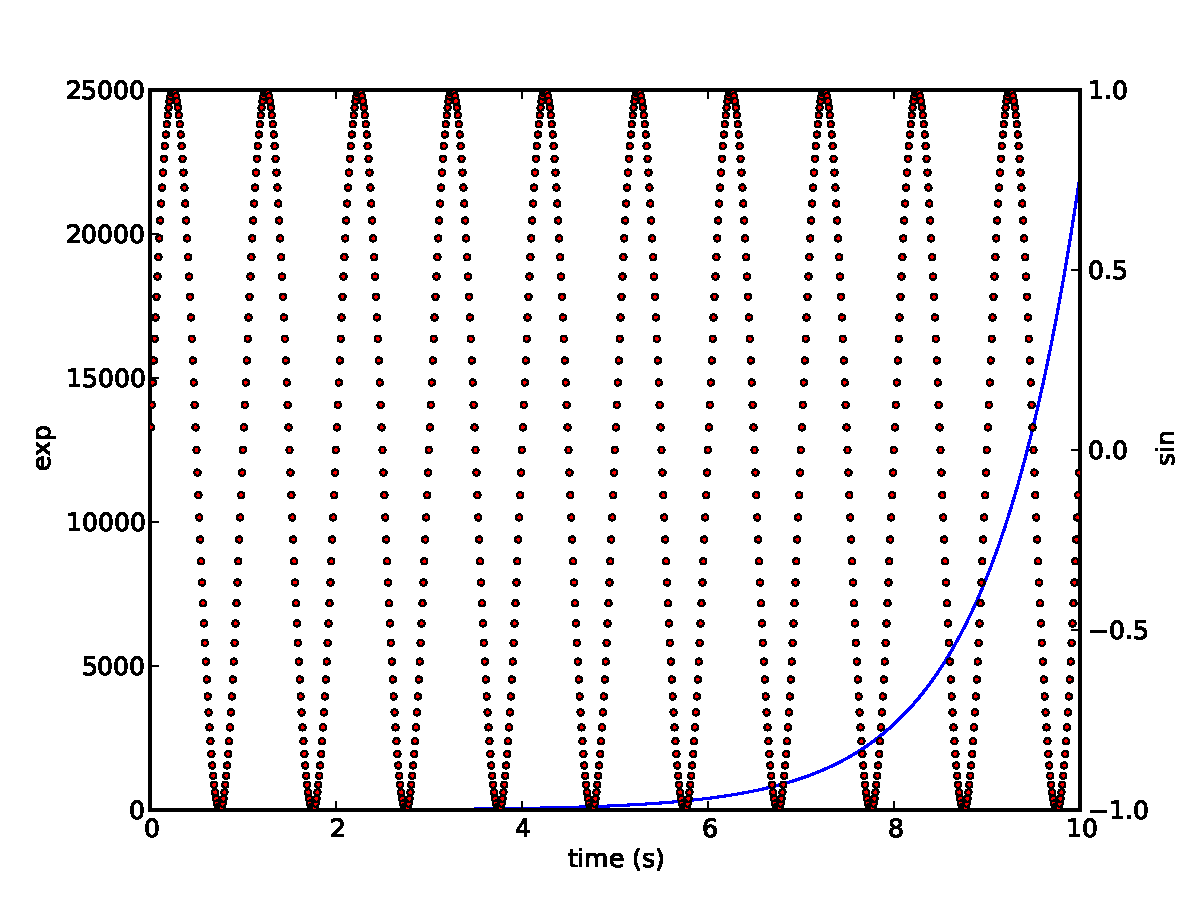
\includegraphics[width=0.5\textwidth]{dynamic/multiaxis.pdf}'
\end{python}
\caption{The functions $\sin$ and $\exp$ together from program~\ref{prog2}.\label{fig:plot2}}
\end{figure}

Some code and its output: The following program produces the plot from Fig.~\ref{fig:plot2}.

\pylabel{prog2}
\VerbatimInput[label=\fbox{\textbf{Program \ref{prog2}:} A plotting example}]{"python/test/plottest01.py"}

\subsection{Image processing}
An example of processing?

\begin{figure}
\centering
\begin{python}
import sys
sys.path.append('python/test')
import matplotlib
import numpy as np
# non-interactive backend
matplotlib.use('PDF') 
## real work done here

import plottest02

## plotting done here
plottest02.saveimages('dynamic/sampleinput.pdf', 'dynamic/sampleoutput.pdf')
## result
print r'\subfigure[]{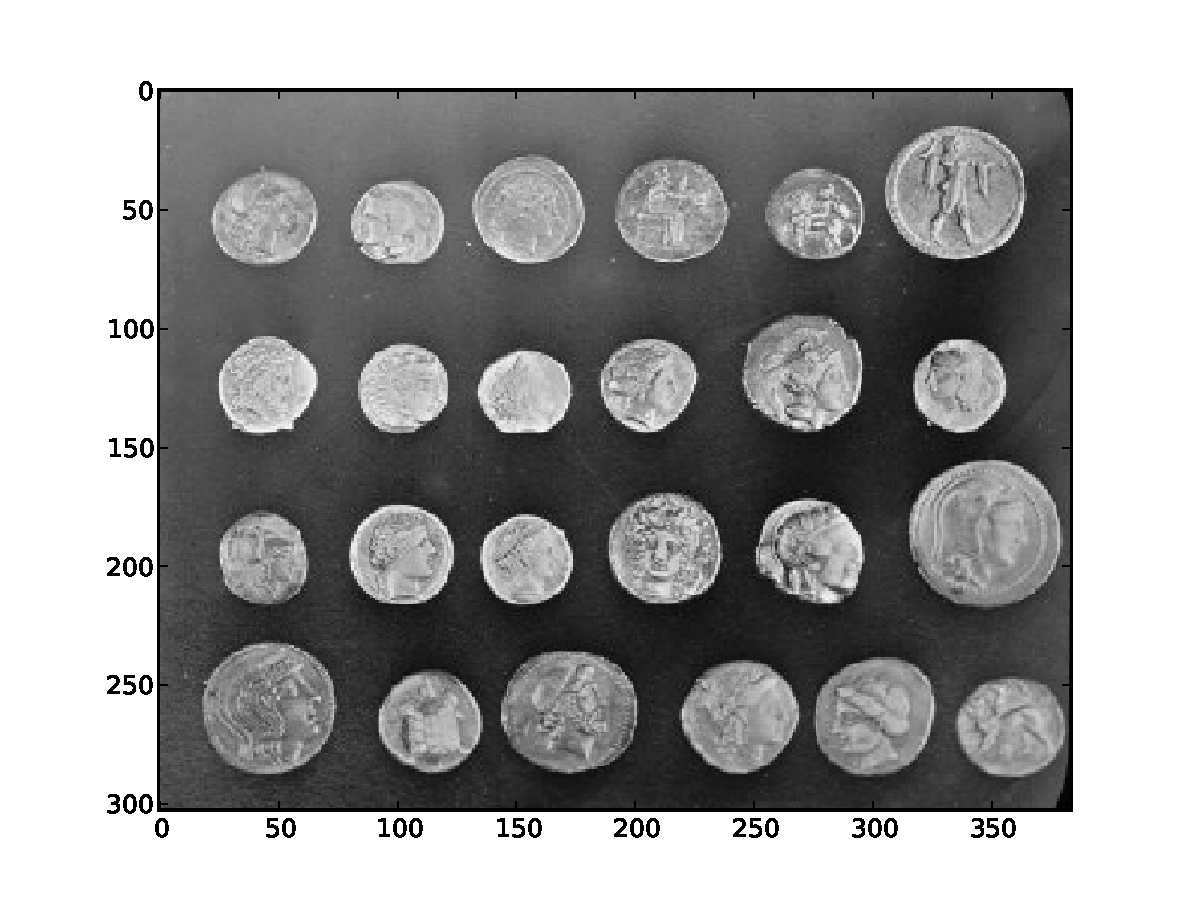
\includegraphics[width=0.45\textwidth]{dynamic/sampleinput.pdf}}'
print r'\subfigure[]{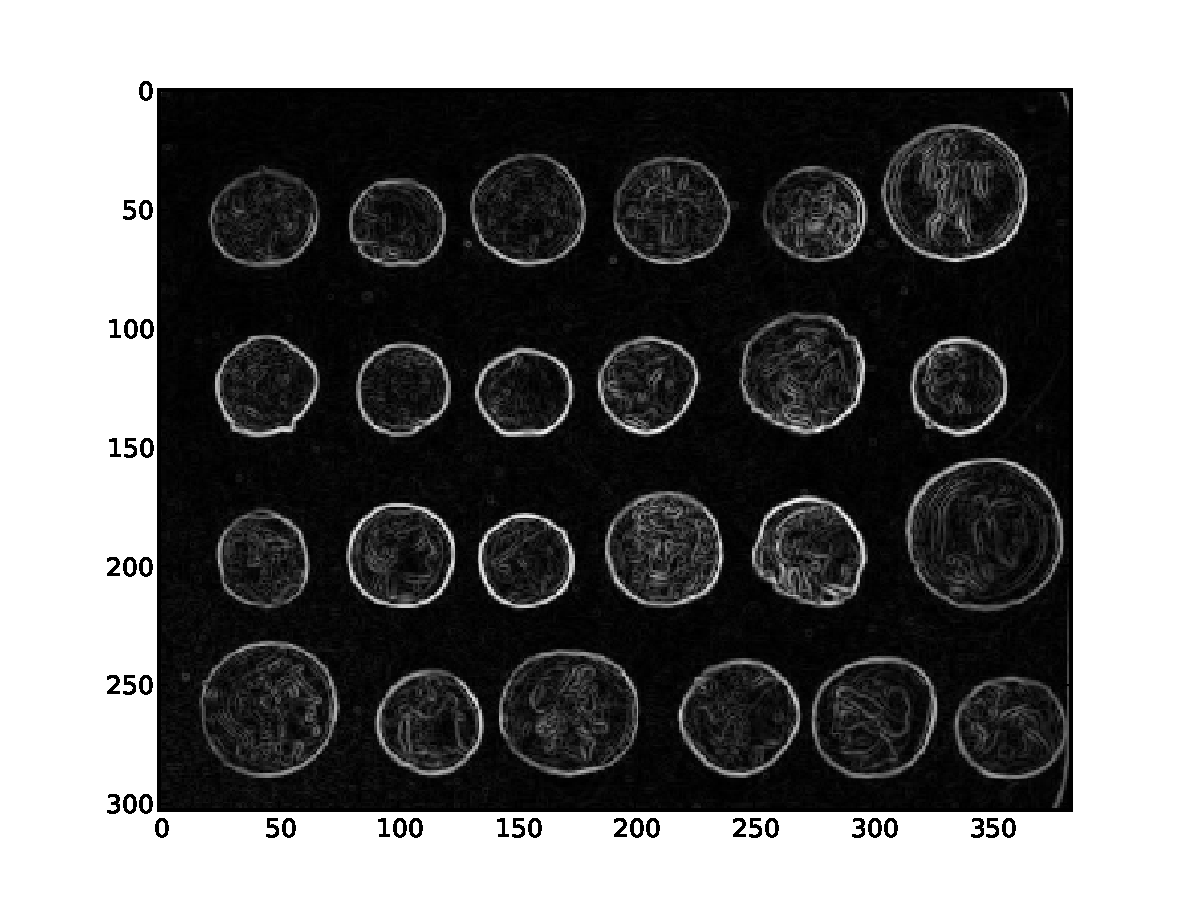
\includegraphics[width=0.45\textwidth]{dynamic/sampleoutput.pdf}}'
\end{python}
\pylabel{prog3}
\VerbatimInput[firstline=2,lastline=13,label=\fbox{\textbf{Program \ref{prog3}:} An image processing example}]{"python/test/plottest02.py"}
\caption{Program~\ref{prog3} and its result.}
\end{figure}





\subsection{Binary image processing}

\subsection{Grey-level segmentation}

\subsection{Discrete geometry}

\subsection{3D image processing}

\section{\Pink and other image-related software}

\subsection{\Pink and numpy}

\subsection{\Pink and scikit}

\subsection{\Pink and VTK}

\subsection{\Pink and ITK}

\section{Exercises}



\chapter{Complementary python tools: numpy, scipy, scikit-image, etc}\label{chap:python-tools}
This chapters describes working with complementary python tools, such as numpy, scipy, the scikits, etc. 

In recent years, python has become a credible replacement for Matlab, thanks to a huge community effort in porting basic numerical facilities to python. Other efforts such as those of Enthought, a company that provides a well-designed distribution of python oriented towards parallel numerical tools, have made python a performance tool suitable for many enterprise-level applications.

The aim of this section is to show how these tools complement \Pink.

\section{Converting from/to numpy}
The {\em lingua franca} of numerical computing under python is numpy. \Pink provides means to swap back and forth between its internal format and numpy arrays.

\pylabel{numpy01}
\VerbatimInput[label=\fbox{\textbf{Program \ref{numpy01}:} Numpy conversion}]{"python/numpy/numpy01.py"}

The plan for future versions of \Pink is to make this conversion automatic and transparent, so that 
for the Python user, \Pink image data is always a numpy array.

\section{Basic numpy usage}


\appendix
%%
%% Installation
%%

\chapter{Compiling and installing \Pink}\label{chap:installing}
Not as difficult as it may seem.



\include{A01_function_reference}

\chapter*{LICENSE}
\markboth{LICENSE}{}
\addcontentsline{toc}{chapter}{LICENSE}

This document \og PINK, A USER MANUAL \fg by Michel Couprie, Laszlo Marak and Hugues Talbot is licensed under a \href{http://creativecommons.org/licenses/by/3.0/}{Creative Commons Attribution 3.0 Unported License}

This means, you are free:

\begin{itemize}
\item to Share — to copy, distribute and transmit the work
\item to Remix — to adapt the work
\item to make commercial use of the work
\end{itemize}

Under the following conditions:

\begin{itemize}
\item Attribution — You must attribute \href{http://creativecommons.org/choose/results-one?q_1=2&q_1=1&field_commercial=y&field_derivatives=y&field_jurisdiction=&field_format=Text&field_worktitle=PINK+A+USER+MANUAL&field_attribute_to_name=Hugues+Talbot&field_attribute_to_url=http%3A%2F%2Fpinkhq.com%2F&field_sourceurl=&field_morepermissionsurl=&lang=en_US&n_questions=3}{PINK A USER MANUAL} to \href{http://pinkhq.com}{Michel Couprie, Laszlo Marak and Hugues Talbot} (with link: \url{http://pinkhq.com/}).
\end{itemize}
  
With the understanding that:

\begin{itemize}
\item Waiver — Any of the above conditions can be waived if you get permission from the copyright holder.
\item Public Domain — Where the work or any of its elements is in the public domain under applicable law, that status is in no way affected by the license.
\item Other Rights — In no way are any of the following rights affected by the license:
  \begin{itemize}
  \item Your fair dealing or fair use rights, or other applicable copyright exceptions and limitations;
  \item The author's moral rights;
  \item Rights other persons may have either in the work itself or in how the work is used, such as publicity or privacy rights.
  \end{itemize}
\end{itemize}

Notice — For any reuse or distribution, you must make clear to others the license terms of this work. The best way to do this is with a link to this web page: \url{http://creativecommons.org/licenses/by/3.0/}

\vfill

\centerline{\hfill
\includegraphics[width=3cm]{drawings/by.pdf}}

%------------------------- Table des symboles ---------------------
%\include{symbol}

%------------------------- table des figures -----------------------
%\thispagestyle{empty}
\addcontentsline{toc}{chapter}{Table of figures}
\listoffigures

%------------------------- table des tables -----------------------
%\thispagestyle{empty}
\addcontentsline{toc}{chapter}{List of tables}
\listoftables

%------------------------- La biblio ------------------------------
%\bibliographystyle{alpha_hut}
\bibliographystyle{apalike}
\addcontentsline{toc}{chapter}{Bibliography}
\bibliography{/Users/talbot/text/TeX/bibs/talbotOnly,/Users/talbot/text/TeX/bibs/talbotOthers}

%------------------------- Index ----------------------------------
%\thispagestyle{empty}
\addcontentsline{toc}{chapter}{Index}
\printindex

\end{document}